\section{Innere Produkte}
In diesem Kapitel sei stets $\mathbb{K}=\mathbb{R}$ oder $\mathbb{K}=\mathbb{C}$.  Wir beschränken uns weiter auf reelle oder komplexe lineare Räume $X$.  Insbesondere im Fall $\K = \Co$ erinnern wir an das komplex-konjugierte
\[\overline{z}=(x,-y)=x-iy\]
einer komplexen Zahl $z=(x,y)=x+iy$, sowie ihren Betrag $\left|z\right|:=\sqrt{zz}=\sqrt{x^2+y^2}$.  Wir betrachten $\R$ als Teilmenge von $\Co$ und erhalten: $z=\overline{z}\Leftrightarrow z\in \R$.
\subsection{Skalarprodukte und Orthogonalität}
\subsubsection{Definition (inneres Produkt)}
\label{5.1.1}
Ein \underline{inneres Produkt} auf $X$ ist eine Abbildung $\langle\cdot ,\cdot \rangle\colon X\times X\rightarrow \K$ mit
\romannum
\begin{enumerate}
\item $\langle\alpha x+\beta y,z\rangle=\alpha \langle x,z\rangle+\beta \langle y,z\rangle$ (\underline{Linearität im 1. Argument})
\item $\langle x,y\rangle=\overline{\langle y,x\rangle}$ (\underline{konjugierte Symmetrie})
\item $\langle x,x\rangle\geq 0$ und Gleichheit genau für $x=0$ (\underline{positive Definitheit})
\end{enumerate}
Für alle $x,y,z\in X,\ \alpha,\beta \in \K$.  Ein linearer Raum mit innerem Produkt heißt auch \underline{Prä-Hilbert-Raum}.\\
Statt innerem Produkt sagt man auch \underline{Skalarprodukt}.
\subsubsection{Bemerkung}
\numbers
\begin{enumerate}
\item Aufgrund der konjugierten Symmetrie ist stets $\langle x,x\rangle\in \R$, während die positive Definitheit $\langle x,x\rangle>0$ für $x\not=0$ garantiert.
\item Ein inneres Produkt ist \underline{Semilinear} im 2. Argument:
\[\phantomsection\label{5.1a}(5.1a)\ \langle x,\alpha y+\beta z\rangle=\overline{\alpha }\langle x,y\rangle+\overline{\beta }\langle x,z\rangle\text{ für alle } x,y,z \in X,\ \alpha, \beta \in \K\]
\item Unter einer \underline{Norm} auf $X$ versteht man die Funktion
\[\|\cdot \|\colon X\rightarrow \R,\ \|x\| :=\sqrt{\langle x,x\rangle}\]
Insbesondere gilt $\|x\|=0\Leftrightarrow x=0$.  Zu jedem $x\not=0$ nennen wir $y:=\frac{1}{\|x\|}x$ den \underline{normierten Vektor} zu $x$, denn $\|y\|=1$.
\end{enumerate}
\subsubsection{Bemerkung (Orthogonalität)}
\begin{enumerate}
\item Die Elemente $x,y\in X$ heißen \underline{orthogonal}, falls $\langle x,y\rangle=0$.  Die resultierende Relation 
\[x \bot y :\Leftrightarrow \langle x,y\rangle=0\]
ist symmetrisch aber nicht transitiv.  Wegen $\langle x,0\rangle=\langle0,x\rangle=0$ ist $0\in X$ orthogonal zu jedem $x\in X$.
\item Die Teilmengen $Y_1,Y_2\subseteq X$ heißen \underline{orthogonal}, insofern
\[\langle y_1,y_2\rangle=0\text{ für alle }y_1\in Y_1,\ y_2\in Y_2\]
\end{enumerate}
\subsubsection{Beispiel (Euklidischer Raum)}
$\R ^n$ mit $\langle x,y\rangle:=\sum _{j=1}^n x_jy_j$, $\|x\|=\sqrt{\sum _{j=1}^nx_j^2}$
\subsubsection{Beispiel (Unitärer Raum)}
$\Co ^n$ mit $\langle x,y\rangle=\sum _{j=1}^n x_j \overline{y_j}$, $n=1$, $\langle i,i\rangle=i\cdot (-i)=1$.
\subsubsection{Beispiel}
\label{5.1.6}
\numbers
\begin{enumerate}
\item Mit sogenannten Gewichten $\omega_1,\dots,\omega_n>0$ ist auch $\langle x,y \rangle_\omega=\sum_{j=1}^n \omega_j x_j \overline{y}_j$ ein inneres Produkt auf $\K^n$ mit induzierter Norm $\|x\|_\omega= \sqrt{\sum_{j=1}^n \omega_j |x_j|^2}$
\item Mit einer stetigen Gewichtsfunktion $\omega\colon[a,b]\rightarrow(0,\infty)$, $a<b$ sind auch die stetigen Funktionen $X=C([a,b],\K)$ ein linearer Raum mit innerem Produkt
\[\phantomsection\label{5.1b}(5.1b)\ \langle x, y\rangle_\omega:=\int_a^b \omega(t)x(t)\overline{y(t)}dt\]
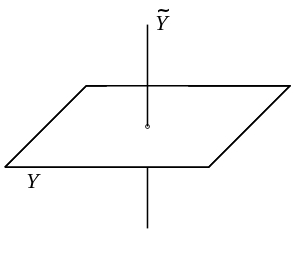
\includegraphics[scale=0.4]{5-1-6.jpg}
\end{enumerate}
\subsubsection{Definition (Orthogonales Komplement)}
Es sei $S \subseteq X$. Dann heißt $S^\bot:=\{x\in X\colon\langle x,y \rangle =0\text{ für alle }y\in S\}$
 das \underline{orthogonale Komplement} von $S$ (in X)
\subsubsection{Beispiel}
\numbers
\begin{enumerate}
\item Es ist $\{0\}^\bot=X$ und $X^{\bot}=\{0\}$
\item Im Raum $X=\R^3$ haben wir in \hyperref[2.5.2]{Beispiel \ref*{2.5.2}} nachgewiesen, dass die Gerade $\tilde{Y}:=\R\begin{pmatrix}1 \\1 \\1\end{pmatrix}$ ein Komplement zur Ebene $Y:=\{x\in X, x_1-x_2+x_3=0\}=\R\begin{pmatrix}1\\1\\0\end{pmatrix}+\R\begin{pmatrix}1\\0\\-1\end{pmatrix}$ ist.
Betrachtet man $\R^3$ als Euklidischen Raum, so ist $\tilde{Y}$ wegen $\left\langle \begin{pmatrix}1 \\1 \\1\end{pmatrix},\begin{pmatrix}1 \\1 \\0\end{pmatrix}\right\rangle=2$ jedoch kein orthogonales Komplement von Y, vielmehr gilt $Y^{\bot}=\R\begin{pmatrix}1 \\-1 \\1\end{pmatrix}$
\end{enumerate}
\subsubsection{Proposition}
\label{5.1.9}
Für jedes $S\subseteq X$ ist $S^{\bot}$ ein Unterraum von $X$ mit $(\spann S)\cap S^{\bot}=\{0\}$.\\
\underline{Beweis}: Es seien $x_1,x_2\in S^{\bot}$ und wir erhalten $\langle \alpha_1 x_1+\alpha_2 x_2,y\rangle=\alpha_1\langle x_1,y\rangle+\alpha_2\langle x_2,y\rangle=0$ für alle $\alpha_1,\alpha_2\in\K$ $y\in S$ dies garantiert $\alpha_1 x_1+\alpha_2 x_2\in S^{\bot}$ und $S^{\bot}$ ist ein linearer Raum.
Weiter sei $x\in\ S^{\bot}$ und $x\in \spann ~S$, d.h. $x=\sum_{i=1}^n \xi_i x_i$ mit Koeffizienten $\xi_i\in \K$ und $x_i\in S$. Dies impliziert $\langle x,x\rangle=\langle \sum_{i=1}^n \xi_i x_i,x\rangle=\sum_{i=1}^n\xi_i \underbrace{\langle x_i,x\rangle}_{=0\text{ weil }x\in S^{\bot}}=0$ und folglich $x=0$.
\subsubsection{Satz}
\label{5.1.10}
Ist $\dim X<\infty$ und $Y$ ein Unterraum von $X$, so gilt
\alphabet
\begin{enumerate}
\item $X=Y\oplus Y^{\bot}$
\item $(Y^{\bot})^{\bot}=Y$
\item $\dim X=\dim Y+\dim Y^{\bot}$
\end{enumerate}
\underline{Beweis (a)}: $Y\cap Y^{\bot}=\{0\}$ gilt nach \hyperref[5.1.9]{Proposition \ref*{5.1.9}}. Es bleibt $X=Y\oplus Y^{\bot}$ zu zeigen. Zu jedem $x\in X$ muss es also $y\in Y$ und $y^{\bot}\in Y^{\bot}$ mit $x=y+y^{\bot}$ geben. Ist $\{y_1, \dots,y_n\}$ eine Orthonormalbasis von $Y$, so definieren wir
\[y:=\sum_{i=1}^m \langle x,y_i\rangle \cdot y_i,\qquad y^{\bot}:=x-y\text{ usw.}\]
\subsubsection{Definition (Orthogonal- und Orthonormalbasis)}
Eine Familie $\mathcal{S} \subseteq X$ heißt
\alphabet
\begin{enumerate}
\item \underline{orthogonal}, falls $\langle x,y\rangle=0$, für alle $x,y\in \mathcal{S}$ $x\neq y$
\item \underline{orthonormal}, falls $\langle x,y\rangle=\begin{cases}1,x=y\\0,x\neq y\end{cases}$, für $x,y\in \mathcal{S}$
\end{enumerate}
Eine Orthogonal- bzw. Orthonormalbasis von X ist eine orthogonale bzw. orthonormale Basis von X.\\
Jede orthonormale Familie ist auch orthogonal.
\subsubsection{Beispiel}
\label{5.1.12}
\numbers
\begin{enumerate}
\item Die Standardbasis $\epsilon_n=\{e_1,\dots,e_n\}$ aus \hyperref[standardbasis]{Beispiel \ref*{standardbasis}} ist eine Orthonormalbasis des Euklidischen Raums $\R^n$ wie auch des unitären Raums $\Co^n$.
\item Die Legendre Polynome $p_n\in P(\R)$, $p_n(t)=\frac{1}{2^n n!} \frac{d^n}{dt^n} (t^2-1)^n$ für $n\in\N_0$ definieren eine orthogonale Familie $\{p_n\}_{n\in\N_0}$ bzgl. dem inneren Produkt (\hyperref[5.1b]{$5.1b$}) aus \hyperref[5.1.6]{Beispiel \ref{5.1.6}(2)} mit $\omega(t)=1$ auf $[-1,1]$
\item Wir definieren die trigonometrischen Funktionen $c_n,s_n\colon[-\pi,\pi]\rightarrow\R$, $c_n(t):=cos(nt)$, $s(t):=sin(nt)$ mit $n\in\N_0$. Dann ist $\mathcal{S}:=\{c_n\}_{n\in\N_0} \cup \{s_n\}_{n\in\N}$ eine orthogonale Familie in $C([-\pi,\pi],\R)$ bezüglich (\hyperref[5.1b]{$5.1b$}) mit $\omega(t)=1$ auf $[-\pi,\pi]$.
\end{enumerate}
\subsubsection{Proposition}
Jede orthogonle Familie $\mathcal{S}\subseteq X$ mit $0\notin\mathcal{S}$ ist linear unabhängig.\\
\underline{Beweis}: Es sei $\{x_1,\dots,x_n\}$ eine endliche Teilfamilie von $\mathcal{S}$ und $\sum_{j=1}^n \xi_j x_j =0$ mit Koeffizienten $\xi_j\in\K$.
Dann resultiert $0=\langle 0,x_k\rangle=\langle\sum_{j=1}^n\xi_j x_j,x_k\rangle=\sum_{j=1}^n \xi_j \langle x_j,x_k\rangle=\xi_k\langle x_j,x_k\rangle$ für alle $1\leq k\leq n$. Wegen $x_k\neq 0$ folgt $\xi_k=0$.\\
Vorteil von Orthonormalbasen: Koordinaten einfach berechenbar
\subsubsection{Proposition}
Ist $\{x_1,\dots,x_n\}$ eine Orthonormalbasis von $X$ so gilt $x=\sum_{j=1}^n \langle x,x_j\rangle x_j$ für alle $x\in X$.\\
\underline{Beweis}: Da $\{x_1,\dots,x_n\}$ orthonormal ist, gilt $\langle x_j,x_k\rangle=\delta_{jk}$ für $1\leq j,k\leq n$. Die Koeffizienten $\xi_j\in\K$ eines beliebigen $x=\sum_{j=1}^n\xi_j x_j \qquad \xi_k=\sum_{j=1}^n\xi_k \underbrace{\langle x_j,x_k\rangle}_{\delta_{jk}}=\langle\sum_{j=1}^n\xi_j x_j,x_k\rangle=\langle x,x_k\rangle$\\
Berechnung von Orthogonal- bzw. Orthonormalbasis aus einer gegebenen Basis: Orthogonalisierungsverfahren von Gram-Schmidt:

\numbers
\begin{enumerate}
\setcounter{enumi}{-1}
\item Es sei eine linear unabhängige Familie $\mathcal{S}:=\{x_1,x_2,x_3,\dots\}$ gegeben auf $X$ mit innerem Produkt $\langle \cdot,\cdot\rangle$
\item Setze $y_1:=x_1$
\item Für $k\geq 1$ definiere
\[\phantomsection\label{5.1c}(5.1c)\ y_{k+1}:=x_{k+1}-\sum _{j=1}^k \frac{\overline{\langle y_j,x_{k+1}\rangle}}{\langle y_j,y_j\rangle}y_j\]
für alle $k\in \mathbb{N}$ solange $x_{k+1}\in\mathcal{S}$.  Wir erhalten aus $\{x_1,x_2,\cdots \}$ eine Familie orthogonaler Vektoren $\{y_1,y_2,\cdots \}=\mathcal{Y}$ und normiert man die Elemente von $\mathcal{Y}$ gemäß
\[\phantomsection\label{5.1d}(5.1d)\ z_k:=\frac{1}{\|y_k\|}y_k,\]
so erhalten wir sogar eine orthonormale Familie.
\end{enumerate}
\subsubsection{Satz}
\label{5.1.15}
Jeder endliche-dimensionale lineare Raum mit innerem Produkt hat eine Orthonormalbasis.\\
\underline{Beweis}: Nach \hyperref[2.4.8]{Satz \ref{2.4.8}} besitzt $X$ eine Basis $\{x_1,\cdots ,x_n\}$.  Auf diese wenden wir obiges Gram-Schmidt-Verfahren an: Es sei $y_1:=x_1$, $y_{k+1}$ für $1\leq k\leq n$ durch \hyperref[5.1c]{$(5.1c)$} gegeben und $\{y_1,\cdots ,y_k\}$ bereits orthogonal.  Wir erhalten dann
\[\langle y_i,y_{k+1}\rangle \stackrel{\hyperref[5.1c]{(5.1c)}}{=}\left\langle y_i,x_{k+1}-\sum _{j=1}^k\frac{\overline{\langle y_j,x_{k+1}}}{\langle y_j,y_j\rangle}y_j\right\rangle = \langle y_i,x_{k+1}\rangle - \left\langle y_i,\sum _{j=1}^k \frac{\overline{\langle y_j,x_{k+1}}}{\langle y_j,y_j\rangle}y_j\right\rangle\]
\[\langle y_i,x_{k+1}\rangle -\sum _{j=1}^k\frac{\langle y_j,x_{k+1}\rangle}{\langle y_j,y_j\rangle}\overbrace{\langle y_i,y_j\rangle}^{\delta_{ij}}\]
\[\langle y_i,x_{k+1}\rangle -\langle y_i,x_{k+1}\rangle = 0\]
dass $y_i$ für alle $1\leq i\leq k$ orthogonal auf $y_{k+1}$ ist.  Wir haben also induktiv eine orthogonale Familie $\{y_1,\cdots ,y_k,y_{k+1}\}$ erzeugt.  Demnach ist $\{y_1,\cdots y_n\}$ eine Orthogonalbasis von $X$.  Die gesuchte Orthonormalbasis $\{z_1,\cdots ,z_n\}$ ergibt sich aus \hyperref[5.1d]{$(5.1d)$}.
\subsubsection{Beispiel (Legendre-Polynome)}
Aufgrund von \hyperref[2.4.4]{Beispiel \ref{2.4.4}} sind die Monome $\mathcal{M}_3:=\{m_0,m_1,m_2,m_3\}$ eine Basis von $P_3(\mathbb{R})$.  Verwenden wir auf $P_3(\R)$ nun das innere Produkt (vgl. \hyperref[5.1b]{$(5.1b)$})
\[\langle p,q\rangle := \int _{-1}^1 p(t)q(t)dt,\]
so ist $\mathcal{M}_3$ wegen $\langle m_k,m_l\rangle = \dfrac{1-(-1)^{k+l+1}}{1+k+l}$ jedoch keine Orthogonalbasis.  Um eine solche zu bestimmen, wenden wir das Gram-Schmidt-Verfahren an.  Zunächst sei dazu $p_0=m_0$ und wegen
\[\langle p_0,m_1\rangle = 0,\ \langle p_0,m_2\rangle = \frac{2}{3},\ \langle p_0,m_3\rangle = 0\]
erhalten wir $p_1=m_1-\dfrac{\langle p_0,m_1\rangle}{\langle p_0,p_0\rangle}p_0=m_1$, also $p_1(t)=t$.  Mittels der Beziehungen
\[\langle p_1,m_2\rangle =0,\ \langle p_1,m_3\rangle =\frac{2}{5}\]
ist weiter $p_2=m_2-\dfrac{\langle p_0,m_2\rangle}{\langle p_0,p_0\rangle}p_0-\dfrac{\langle p_1,m_2\rangle}{\langle p_1,p_1\rangle}p_1=m_2-\dfrac{\langle p_0,m_2\rangle}{\langle p_0,p_0\rangle}p_0$, also $p_2(t)=t^2-\frac{1}{3}$.  Ebenso erhält man $p_3(t)=t^3-\frac{3}{5}t$ und hieraus ergibt sich die Orthonormalbasis $\{q_0,q_1,q_2,q_3\}$ des $P_3(\R)$ mit
\[q_0(t)\equiv\sqrt{\frac{1}{2}},\ q_1(t)=\sqrt{\frac{3}{2}}t,\ q_2(t)=\frac{3}{2}\sqrt{\frac{5}{2}}(t^2-\frac{1}{3}),\ q_3(t)=\frac{5}{2}\sqrt{\frac{7}{2}}(t^3-\frac{3}{5}t)\]
Fordert man nicht die Normierung $\langle q_k,q_k\rangle = 1$, sondern $q_k(1)=1$, so ergibt sich durch Multiplikation der $p_k$ mit einem geeigneten Faktor, dass
\[q_0(t)\equiv 1,\ q_1(t)=t,\ q_2(t)=\frac{1}{2}(3t^2-1),\ q_3(t)=\frac{1}{2}(5t^3-3t);\]
dies sind die Legendre-Polynome aus \hyperref[5.1.12]{Beispiel \ref{5.1.12}(2)}
\subsection{Adjungierte Abbildungen}
Sei $X$ ein linearer Raum über $\K$ mit innerem Produkt $\langle \cdot ,\cdot\rangle$.  Eine lineare Abbildung $S\colon X\rightarrow \K$ heißt \underline{Funktional}.  Mit gegebenem $y\in X$ definieren wir das Funktional $y'\colon X\rightarrow \K$ durch
\[\phantomsection\label{5.2a}(5.2a)\ y'(x)\colon =\langle x,y\rangle\text{ für alle } x\in X\]
Aufgrund von \hyperref[5.1.1]{Definition \ref{5.1.1}(i)} gilt nämlich $y'(\alpha _1x_1+\alpha _2x_2)=\langle \alpha _1x_1+\alpha _2x_2,y\rangle = \alpha _1\langle x_1,y\rangle +\alpha _2\langle x_2,y\rangle = \alpha _1 y'(x_1)+\alpha _2 y'(x_2)$ für alle $\alpha _1,\alpha _2\in \K ,\ x_1,x_2\in X$, also $y'\in L(X,\K)$
\subsubsection{Satz (Riesz'scher Darstellungssatz)}
\label{5.2.1}
Ist $\dim X<\infty$, so gibt es zu jedem Funktional $S\in L(X,\K)$ ein eindeutiges $y\in X$ mit $Sx=\langle x,y\rangle$ für alle $x\in X$, d.h. $S=y'$.\\
\underline{Beweis}: Nach \hyperref[5.1.15]{Satz \ref{5.1.15}} gibt es eine Orthonormalbasis $\{x_1,\cdots ,x_n\}$ von $X$.
\Romannum
\begin{enumerate}
\item \underline{Existenz}: Zu beliebig gegebenem $S\in L(X,\K)$ sei
\[\phantomsection\label{5.2b}(5.2b)\ y\colon = \sum _{i=1}^n \overline{Sx_i}x_i\in X\]
und es gilt
\[\langle x_j,y\rangle \stackrel{\hyperref[5.2b]{(5.2b)}}{=} \left\langle x_j,\sum _{i=1}^n\overline{Sx_i}x_i\right\rangle =\sum _{i=1}^n \overline{\overline{Sx_i}}\overbrace{\langle x_j,x_i\rangle}^{\delta_{ij}}=Sx_j\text{ für }1\leq j\leq n\]
Damit stimmen $S$ und $y'$ auf einer Basis von $X$ überein, weshalb \hyperref[lfortsetzung]{Satz \ref{lfortsetzung}(a)} sofort $S=y'$ garantiert.
\item \underline{Eindeutigkeit}: Um nachzuweisen, dass obiges $y$ aus \hyperref[5.2b]{$(5.2b)$} eindeutig bestimmt ist, erfülle auch $z\in X$ die Beziehung $Sx=\langle x,y\rangle = \langle x,z\rangle $ für alle $x\in X$.  Dies impliziert $\langle x,y-z\rangle = 0$ für alle $x\in X$ und damit $y-z=0$
\end{enumerate}
Nun seien $T\in L(X)$, $y\in X$.  Wir definieren $S_y\colon X\rightarrow \K$
\[S_yx\colon =\langle Tx,y\rangle\]
und es folgt sofort $S_y\in L(X,\K)$.  Bei festem $T$ gibt es nach \hyperref[5.2.1]{Satz \ref{5.2.1}} zu jedem $y\in X$ ein eindeutiges $y_0\in X$ mit $S_yx=\langle x,y_0\rangle$ für alle $x\in X$.  Wir bezeichnen diese Zuordnung $y\mapsto y_0$ mit $T'$ und die entsprechende Abbildung $T' \colon X\rightarrow X$ ist festgelegt durch
\[\langle Tx,y\rangle = \langle x,T' y\rangle\text{ für alle }x,y\in X\]
Gegeben $T=L(X)$, $y\in X$.  Wir definieren:
\[S_yx:=\langle Tx,y\rangle\]
und mittels \hyperref[3.1a]{$(3.1a)$}, sowie \hyperref[5.1.1]{Definition \ref{5.1.1}$(i)$} folgt sofort $S_y\in L(X,\K)$.  Bei festen $T\in L(X)$ gibt es nach \hyperref[5.2.1]{Satz \ref{5.2.1}} dann ein eindeutig bestimmtes $y_0\in X$mit $S_yx=\langle x,y_0\rangle$.  Wir bezeichnen diese Zuordnung $y\mapsto y_0$ mit $T'$ und die Abbildung $T'\colon X\rightarrow X$ ist festgelegt durch $\langle Tx,y\rangle=\langle x,T'y\rangle$ für alle $x,y\in X$.  Aufgrund von \hyperref[5.1.1]{Definition \ref{5.1.1}} erhalten wir mit beliebigen $x_1,x_2\in X$,$\alpha _1,\alpha _2\in \K$, dass
\[\langle x,T'(\alpha _1x_1+\alpha _2x_2)\rangle =\langle Tx,\alpha _1x_1+\alpha _2x_2\rangle = \overline{\alpha _1}\langle Tx,x_1\rangle +\overline{\alpha _2}\langle Tx,x_2\rangle=\overline{\alpha _1}\langle x,T'x_1\rangle + \overline{\alpha _2}\langle x,T'x_2\rangle\]
\[\langle x,\alpha _1T'x_1+\alpha _2T'x_2\rangle\]
Damit ist $T'\in L(X)$.
\subsubsection{Definition (adjungierte Abbildung)}
Die zu $T\in L(X)$ \underline{adjungierte Abbildung} $T'\in L(X)$ ist definiert durch
\[\phantomsection\label{5.2c}(5.2c)\ \langle Tx,y\rangle = \langle x,T'y\rangle \text{ für alle } x,y\in X\]
Man beachte, dass $T'$ von konkret auf $X$ verwendete inneren Produkt abhängt.
\subsubsection{Bemerkung}
Direkt aus \hyperref[5.2c]{$(5.2c)$} folgt
\numbers
\begin{enumerate}
\item Die Abbildung $\cdot '\colon L(X)\rightarrow L(X)$ ist \underline{semilinear}, d.h.
\[(\alpha _1T_1+\alpha _2T_2)'=\overline{\alpha _1}T'_1+\overline{\alpha _2}T'_2\text{ für }\alpha _1,\alpha _2\in \K, T_1,T_2\in L(X)\]
und erfüllt $T''=T$, sowie $(ST)'=T'S'$ für $S,T\in L(X)$
\item Für $T\in GL(X)$ ist auch $T'\in GL(X)$ mit
\[(T')^{-1}=(T^{-1})'\]
\end{enumerate}
\subsubsection{Beispiel (Transponierte)}
Es sei $X=\R ^n$ (Euklidisch) ausgestattet mit der Standardbasis $\mathcal{E}_n=\{e_1,\cdots ,e_n\}$ und $A\in \R ^{n\times n}$ die darstellende Matrix von $T\in L(X)$, d.h. $Tx=Ax$ für alle $X\in \R ^n$.  Bezeichnet dann $A'\in \R ^{n\times n}$ die darstellende Matrix von $T'$, so ist
\[a'_{ij}=\left\langle e_i,\begin{pmatrix}a'_{1j}\\ \vdots \\ a'_{nj}\end{pmatrix}\right\rangle = \langle e_i,T'e_j\rangle\stackrel{\hyperref[5.2c]{(5.2c)}}{=}\langle Te_i,e_j\rangle =\left\langle \begin{pmatrix}a_{1i}\\ \vdots \\ a_{ni}\end{pmatrix},e_j\right\rangle = a_{ij} \text{ für alle }1\leq i,j\leq n.\]
Folglich ist die adjungierte Abbildung $T'$ in Euklidischen Räumen gerade durch die Transponierte $A'=A^T$ gegeben (vergleiche \hyperref[3.2.3]{Beispiel \ref{3.2.3}}).
\subsubsection{Beispiel (Hermite'sche)}
\label{5.2.5}
Im unitärer Raum $\Co ^n$ mit seiner Standardbasis $\mathcal{E}_n$ ergibt sich entsprechend:
\[\overline{a'_{ij}}=\left\langle e_i,\begin{pmatrix}a'_{1j}\\ \vdots \\ a'_{nj}\end{pmatrix} e_i,T'e_j\right\rangle \stackrel{\hyperref[5.2c]{(5.2c)}}{=}\langle Te_i,e_j\rangle = \left\langle \begin{pmatrix}a_{1i}\\ \vdots \\ a_{ni}\end{pmatrix},e_j\right\rangle=a_{ji}\text{ für alle } 1\leq i,j\leq n\]
und folglich $a'_{ij}=\overline{a_{ji}}$.  Für die adjungierte Abbildung in unitären Räumen ist also $A'=A^*$ mit der sogenannten \underline{Hermite'schen}
\[A^*=\overline{(A^T)}=(\overline{a_{ji}})_{1\leq i,j\leq n}\]
\subsubsection{Satz}
Ist $\dim X<\infty$ und $T\in L(X)$, so gilt
\[N(T')=R(T)^\bot\ \ \mathrm{rk}T=\mathrm{rk}T'\]
\underline{Beweis}: Wir erhalten
\[N(T')=\{x\in X\colon T'x=0\}=\{x\in X\colon \langle y, T'x\rangle =0\text{ für alle }y\in X\}\]
\[\stackrel{\hyperref[5.2c]{(5.2c)}}{=}\{x\in X\colon \langle Ty,x\rangle =0\text{ für alle } y\in X\}=R(T)^\bot\]
Mit \hyperref[5.1.10]{Satz \ref{5.1.10}(c)}, der eben gezeigten Aussage und \hyperref[dimension]{Satz \ref{dimension}}
\[\mathrm{rk}T=\dim R(T)=\footnotemark\dim X-\dim R(T)^\bot =\dim  X-\dim N(T')=\dim R(T')=\mathrm{rk}T'\]
\footnotetext{gilt wegen: $X=Y\oplus Y^\bot\\ \dim X=\dim Y+\dim Y^\bot$}
\subsection{Sebstadjungierte Abbildungen}
Wieder sei $X$ ein linearer Raum mit inneren Produkt $\langle \cdot ,\cdots \rangle$
\subsubsection{Definition (Selbstadjungiert)}
Eine Abbildung $T\in L(X)$ heißt \underline{selbstadjungiert}, falls gilt $T=T'$, d.h.
\[\phantomsection\label{5.3a}(5.3a)\langle Tx,y\rangle =\langle x,Ty\rangle \text{ für alle }x,y\in X\]
\subsubsection{Beispiel (Euklidischer Raum)}
Auf dem Euklidischen Raum $\R ^n$ ist eine Abbildung $T\in L(X)$ genau dann selbstadjungiert, falls ihre darstellende Matrix $T_{\mathcal{E}_n}=A$ \underline{symmetrisch} ist, d.h. $A=A^T$
\[\text{z.B.}\ \begin{pmatrix}1 & 2\\ 2 & 1\end{pmatrix},\begin{pmatrix}1 & 3\\ 3 & 2\end{pmatrix}, \begin{pmatrix}1 & 2\\ 3 & 4\end{pmatrix}\text{ nicht.}\]
\subsubsection{Beispiel (unitärer Raum)}
In einem unitären Raum $\Co ^n$ ist $T\in L(\Co ^n)$ dann und nur dann selbstadjungiert, wenn $A=T_{\mathcal{E}_n}$ Hermite'sch ist (vergleiche \hyperref[5.2.5]{Beispiel \ref{5.2.5}}), d.h. $A=A^*$.
\addtocounter{subsubsection}{1}
\subsubsection{Satz}
Es sei $\dim X<\infty$.  Ist $T\in L(X)$ selbstadjungiert, so gilt:
\alphabet
\begin{enumerate}
\item $\sigma (T)\subseteq \R$
\item Es gibt eine Orthonormalbasis von $X$ aus Eigenvektoren von $T$
\end{enumerate}
\subsubsection{Bemerkung}
Auf Matrizen bezogen besagt dies gerade, dass symmetrische und Hermite'sche Matrizen reelles Spektrum haben und der Raum $\K ^n$ eine Orthonormalbasis aus Eigenvektoren besitzt.
\underline{Beweis}: 
\begin{enumerate}
\item Es sei $\lambda \in \K$ ein Eigenwert von $T$ mit zugehörigen Eigenvektor $x\in X$.  Da $T$ selbstadjungiert ist, gilt
\[\lambda \langle x,x\rangle = \langle \lambda x,x\rangle \stackrel{\hyperref[4.2a]{(4.2a)}}{=}\langle Tx,x\rangle = \langle x,Tx\rangle \stackrel{\hyperref[4.2a]{(4.2a)}}{=} \langle x,\lambda x\rangle = \overline{\lambda}\langle x,x\rangle\]
und wegen $x\not=0$ folgt $\lambda =\overline{\lambda}$, also $\lambda \in \R$.
\item Induktion über $n=\dim X$.  Für $n=1$ ist nichts nachzuweisen.  Für $n>1$ gilt den Fundamentalsatz der Algebra
\[\chi _T(t)=\prod _{i=1}^n(\lambda _i-t)\text{ mit }\lambda _i\in \Co\]
und wegen \hyperref[4.3.3]{Satz \ref{4.3.3}} ist jedes $\lambda _i$ Eigenwert von $T$;
Aussage (a) garantiert sogar $\lambda _i\in \R$.  Es sei nun $x_1$ ein normierter Eigenvektor zu $\lambda _1$ und $X_1=(\spann \{x_1\})^\bot$.  Mittels \hyperref[5.1.10]{Satz \ref{5.1.10}(c)} ist dann $\dim X_1=n-1$.  Für jedes $x\in X_1$ ist dann
\[\langle x_1,Tx\rangle \stackrel{\hyperref[5.3a]{(5.3a)}}{=}\langle Tx_1,x\rangle \stackrel{\hyperref[4.2a]{(4.2a)}}{=}\lambda _1\overbrace{\langle x_1,x\rangle}^0=0\]
d.h. $Tx\in X_1$.  Wir haben damit gezeigt, dass $X_1$ invariant unter $T$ ist.  Damit induziert $T\in L(X)$ eine selbstadjungierte Abbildung $T_1\colon =T\mid _{X_1}\in L(X_1)$.  Nach Induktionsvoraussetzung gilt es eine Orthonormalbasis $\mathcal{X}_1\colon =\{x_2,\cdots ,x_n\}$ von $X_1$ aus nomierten Eigenvektoren $x_i$ von $T$.  Da jeder Eigenvektor von $T_1$ auch Eigenvektor von $T$ ist, muss $\{x_1,x_2,\cdots ,x_n\}$ eine Orthonormalbasis von $X$ sein.
\end{enumerate}
\subsubsection{Korollar}
Jede selbstadjungierte Abbildung ist diagonalisierbar.
\underline{Beweis}: Wähle Basis aus Eigenvektoren.